\documentclass[10pt]{article}
\usepackage[utf8]{inputenc}
\usepackage{multicol}
\usepackage{graphicx}
\usepackage{amsmath}
\usepackage{amsfonts}
\usepackage{mathtools}
\usepackage{siunitx}
\usepackage{braket}
\usepackage{parskip}
\usepackage{wrapfig}
\usepackage[letterpaper, portrait, margin=1in]{geometry}
\renewcommand{\baselinestretch}{0.95}
\title{Quantum HW7}
\author{bellenchia}
\date{March 2019}
\begin{document}
\maketitle
\section*{24.) Scaling in Hydrogenic Atoms}

From chapter 4, we obtained a general result for the wave function of an Electron bound to the nucleus of a Hydrogen atom, which allowed us to write the energy of such states as follows;\\
$E_n=-[\frac{m}{2\hbar^2}(\frac{e^2}{4\pi\epsilon_0})^2]\frac{1}{n^2}.$\\

Consider instead, the potential arising from the interaction between an electron and a nucleus of charge $+Ze$. Coulomb's Law tells us that;\\

$F(r)=\frac{1}{4\pi\epsilon_0}\frac{|q_1||q_2|}{r^2}$, and in our case; $F(r)=\frac{1}{4\pi\epsilon_0}\frac{Ze^2}{r^2}$\\

Integrating this to find our function of potential; we have $-{\displaystyle\int}F(r)dr=V(r)=\frac{-1}{4\pi\epsilon_0}\frac{Ze^2}{r}$\\

Thus, our solution to the Schroedinger equation is changed only by a constant of Z in our potential, resulting in the following equation;\\ $E_n=-[\frac{m}{2\hbar^2}(\frac{Ze^2}{4\pi\epsilon_0})^2]\frac{1}{n^2}$.\\

\textbf{a) } Modelling $C^{+5}$ using our hydrogen model, we can evaluate the energy needed to release the (1s) electron, shown in the following Mathematica notebook.\\
The data value online, ~284eV, is the binding energy for \textbf{neutral} Carbon, meaning there are more electrons bound to the nucleus. The more electrons occupying the atom, the more repulsive forces each electron experiences from one another. In our model, the $C^{+5}$ has only one electron, the lack of repulsive forces from other electrons means more energy is required to release it from the atom.\\


\begin{center}
    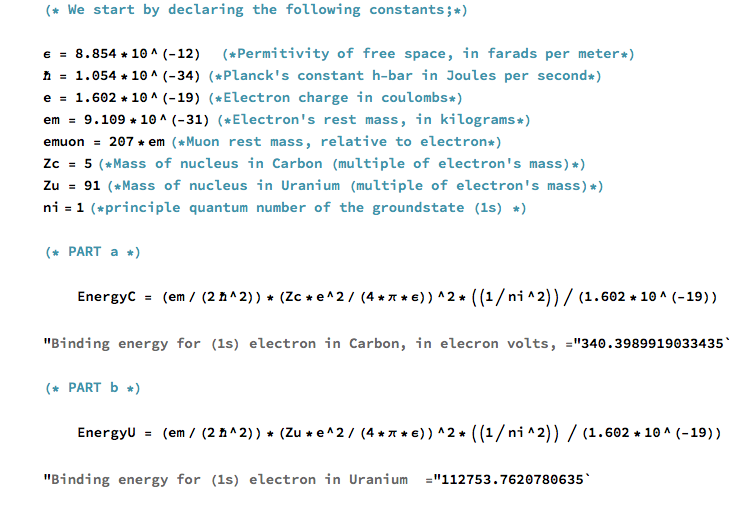
\includegraphics[width=0.9\linewidth]{parts_a_b.png}
\end{center}

\textbf{c)} The estimate for Carbon is off by aboout 200 eV's $(489-284)$ where the Uranium estimate is off by a ~20,000 $(131821-112753)$. An atom like Uranium has quite a massive nucleus (it's atomic mass is ~230amu),  regarding binding energies, the greater the atomic mass (not just protons, but neutrons as well), the greater the binding energy.

\textbf{d)}


Our generalized result for the Hydrogen atom evaluated for $n=1$,$l=0$,$m=0$ is $\psi(r,\theta,\phi)_{100}=\frac{1}{\sqrt{\pi a}}e^{-r/a}$ where $a$ is the Bohr radius of the particle in question. The Bohr's radius is given by the following relation; $a=\frac{4\pi\epsilon_0\hbar^2}{m E^2}$\\

Finding the probability of our electron being inside the proton requires integrating the square modulus of our wave funcion over the region of space in which the proton inhabits. This radius is approximately $r_p=8.78\cdot10^{-10}m$. The following code shows our results.\\
\begin{center}
    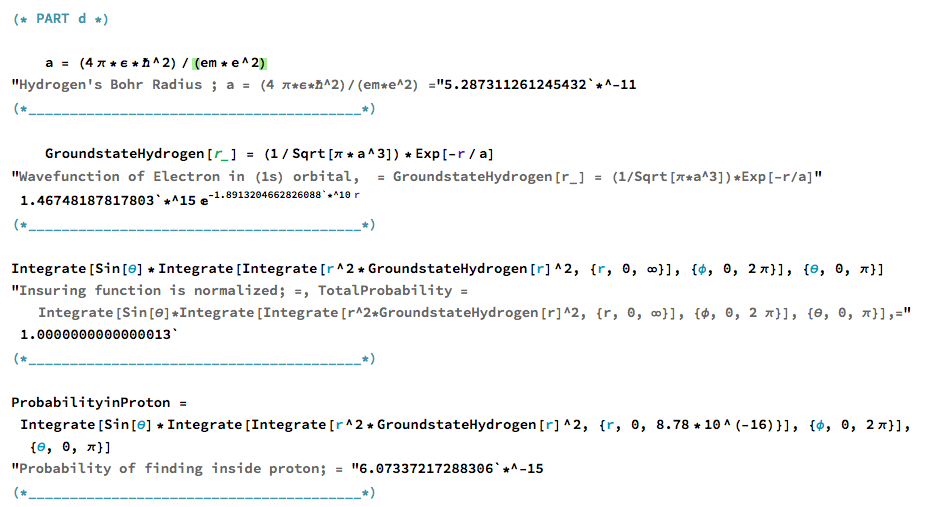
\includegraphics[width=0.9\linewidth]{partd2.png}
\end{center}

\textbf{e) } 
%The entirety of this exercise is contained within the following Mathematica notebook;\\

\begin{center}
    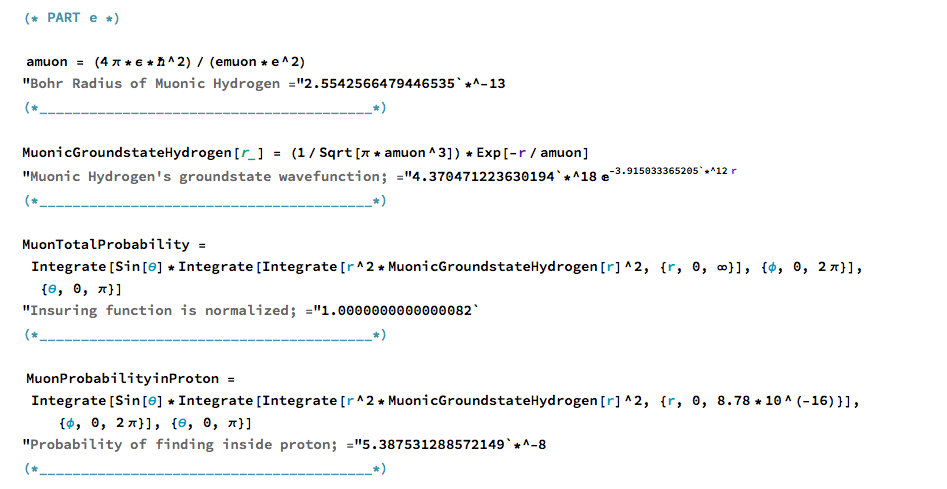
\includegraphics[width=0.9\linewidth]{parte.png}
\end{center}

The probability of finding the electron inside the proton is on the order of $10^{-15}$ whereas the probability of finding a Muon inside the proton is on the order or $10^{-8}$. The relative likelihood for a Muon is on the order of $10^{7}$ times more probable than the electron.

\section*{25.) Interaction of Light with Matter Basics}
We're given an electric field of the form $\hat{E}(\hat{r}),t=\hat{z}E_0cos(kx-\omega t)$\\

\textbf{a)}  To find the phase difference of a \textit{visible light wave} at either end of a Hydrogen atom, we use the Bohr radius $a=0.529\times10^{-10}m$ and $k=2\pi/\lambda$ where $\lambda$ is in the visible spectrum, approximately $400-700\times10^{-9}m$.\\

$\Delta\phi=[kx_2-kx_1]=2\pi[\frac{a}{\lambda}]\approx\frac{\pi}{5000}$, this difference can be easily neglected since the contribution to the phase is so small in this frequency range.\\

\textbf{ b ) } We know light intensity, which is the magnitude of the Poynting vector $\vec{S}$ is related to the electric field in the following way $|\vec{S}|=|\vec{E}\times\vec{H}|=\frac{|\vec{E}|^2}{Z_0}$ where the impedence of free space $Z_0$ is roughly $376.7$ ohms.\\

$I=|S|=\frac{|\vec{E}|^2}{Z_0}\Rightarrow |E|=\sqrt{1000Z_0}=~613.75 V/m$.\\

Since Electrons in hydrogen atoms occupy space in the order of angstroms, this field is minuscule. \\

\textbf{ c) } To calculate the necessary electric field for Barrier supression, solve for when $V_{coulomb}=V_{field}$\\

$ezE_0=-\frac{1}{4\pi\epsilon_0}\frac{1}{z}$\\

$\Rightarrow z=\pm\sqrt{\frac{1}{4\pi\epsilon_0E_0}}$\\

Plug this into the equation $V_{coulomb}+V_{field}=-13.6ev$\\

We get $\frac{eE_0+1}{(-13.6eV)}=\sqrt{4\pi\epsilon_0E_0}$\\

Which leads to the equation \\

$\frac{e^2 E_0^2-2eE_0+1}{(13.6eV)^2}=4\pi\epsilon_0 E_0$\\

This can be solved to find the necessary field.\\


\section*{26.) Atomic Dipoles}

\textbf{a)} The dipole matrix element between the (1s) to (2s) states is as follows; \\

$|\braket{\Psi_{100}|e\cdot\hat{z}|\psi_{200}}|^2=|\braket{R_{10}(r)Y_0^0|ercos\theta|R_{20}(r)Y_0^0}|^2=e^2|{\displaystyle\int_0^\infty}r^3R_{20}(r)R_{21}(r)dr{\displaystyle\int_0^\pi}sin\theta cos\theta d\theta {\displaystyle\int_0^{2\pi}}d\phi|^2$\\

Since $ {\displaystyle\int_0^\pi}sin\theta cos\theta d\theta=0$, we have $|\braket{\Psi_{100}|e\cdot\hat{z}|\psi_{200}}|^2=0$, this is verified by Mathematica\\

\begin{center}
    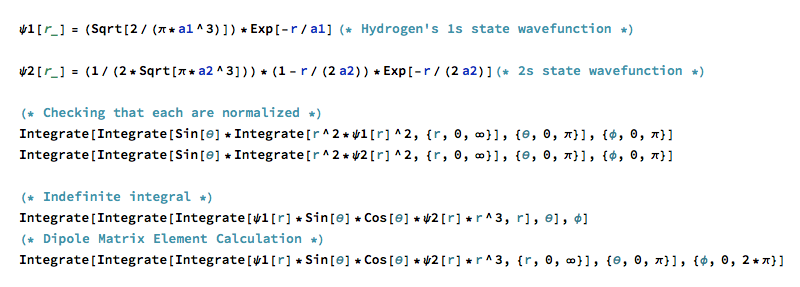
\includegraphics[width=0.9\linewidth]{26a.png}
\end{center}


\textbf{b)} We seek to generally find the Dipole matrix element for the (2p) to all it's m=-1,0,1 states;\\

$|\braket{\Psi_{200}|ercos\theta|\psi_{21m}}|^2=|\braket{R_{20}Y_1^0|ercos\theta|R_{21}Y_1^m}|^2=$\\

$e^2| {\displaystyle\int_0^\infty}r^3R_{20}(r)R_{21}(r)dr {\displaystyle\int_0^\pi} cos\theta sin\theta P_1^m(cos\theta) d\theta {\displaystyle\int_0^{2\pi}}e^{im\phi}d\phi|^2$\\

Since  ${\displaystyle\int_0^{2\pi}}e^{im\phi}d\phi|^2=0$ for $m\neq0$, we know that $|\braket{\Psi_{200}|e\cdot\hat{z}|\psi_{21m}}|^2=0$ for $m=-1,1$\\

To evaluate the $m=0$ case, we must acknowledge $Y_1^0=\sqrt{\frac{3}{4\pi}}cos\theta$. We obtain;\\

$e^2| {\displaystyle\int_0^\infty}r^3R_{20}(r)R_{21}(r)dr {\displaystyle\int_0^\pi} cos\theta sin\theta \sqrt{\frac{3}{4\pi}}cos\theta d\theta {\displaystyle\int_0^{2\pi}}d\phi|^2=e^2|(-3\sqrt{3}a_2)(\frac{1}{\sqrt{3}})(2\pi)|^2=36\pi e^2 a_2^2$\\

The rough work was done by Mathematica;\\
\begin{center}
    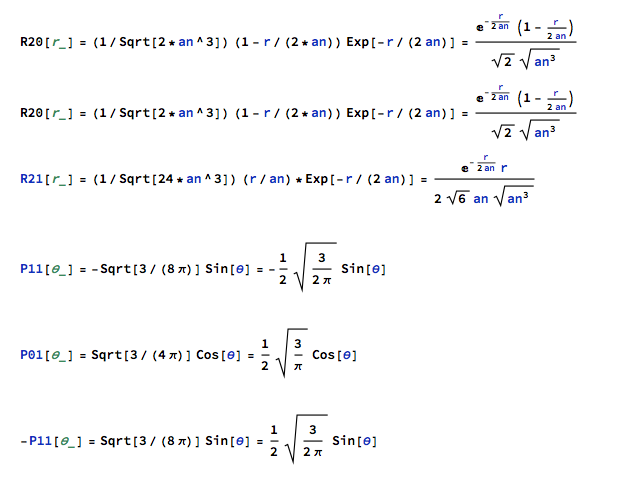
\includegraphics[width=0.9\linewidth]{26fns.png}
\end{center}


\begin{center}
    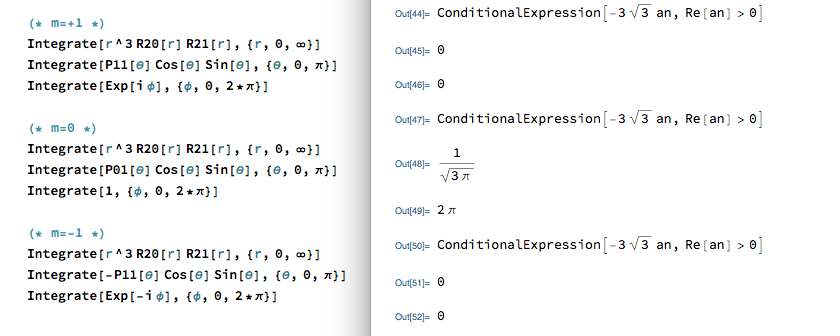
\includegraphics[width=0.9\linewidth]{26ints.png}
\end{center}



\textbf{ c) } Considering a state 

$\ket{\Psi}=\frac{1}{\sqrt{2}}e^{-iE_1t/\hbar}\ket{\psi_{100}}+\frac{1}{\sqrt{2}}e^{-iE_2t/\hbar}\ket{\psi_{210}}$\\

We know that for hydrogen, $E_n=\frac{E_1}{n^2}\Rightarrow E_1=4E_2$, thus the two states in which $\ket{Psi}$ is a superposition exhibit "beats," like sound wave interference of different frequencies which are multiples of the same harmonic.\\

Thus, in regular intervals the $\ket{\Psi}$ is either completely in one state or the other.\\
We calculated previously that these states' transition have a nonzero Dipole matrix element. This means that energy is released in the form of electromagnetic waves.\\


\end{document}
